\section{Theorie}
Im Veruch soll der Zeeman Effekt untersucht werden. Dieser beschreibt die Aufspaltung der
von einem Atom emittierten Spektrallinien, wenn dieses einem äußeren Magnetfeld unterworfen
ist. Hierzu wird die rote und die blaue Linie einer Cadmiumlampe (Cd-Lampe) im Speziellen
untersucht.
\subsection{Magnetische Momente}
Ein Elektron im Atom besitzt zwei unterschiedliche Drehimpulse. Zum einen den Bahndrehimpuls
$\vec{l}$ und zum anderen den Eigendrehimpuls $\vec{s}$, der als Spin bezeichnet wird.
Die Beträge beider Größen berechnen sich wie folgt:
\begin{align*}
    |\vec{l}| =& \sqrt{l(l+1)}\hbar \ \ l =& {0, 1, 2, ..., n-1}\\
    |\vec{s}| =& \sqrt{s(s+1)}\hbar \ \ s =& \frac{1}{2}.
\end{align*}
Dabei beschreiben $l$ und $s$ jeweils die Drehimpuls-, beziehungsweise Spinquantenzahl
und $\hbar$ ist das Planck'sche Wirkungsquantum.
Da Elektronen eine Ladung besitzen, entstehen durch ihre Drehimpulse die dazugehörigen
magnetische Momente $\vec{\mu_l}$ und $\vec{\mu_s}$.
Diese lassen sich mit Hilfe des Bohr'schen Magnetons
\FloatBarrier
\begin{align*}
    \mu_B := -\frac{1}{2}e_0\frac{\hbar}{m_0}
\end{align*}
wie folgt berechnen:
\begin{align*}
    \vec{\mu}_l =& \mu_B\sqrt{l(l+1)}\vec{l}_e\\
    \vec{\mu}_s =& \mu_B \, g_s \sqrt{s(s+1)} \vec{s}_e .
\end{align*}
Beide Momente besitzen einen Landé-Faktor ($g_s$). Er beschreibt die Stärke der Kopplung des
Spins, beziehungsweise des Bahndrehimpulses an das magnetische Moment. Im Falle von
$\vec{\mu}_l$ beträgt der Landé-Faktort jedoch eins und wurde deshalb nicht aufgeführt.
Im Falle von $\vec{\mu}_s$ beträgt er in etwa zwei.
Im Falle, dass die Spinquantenzahl $s$ $\frac{1}{2}$ und $l$ 1 beträgt, so ist
$\vec{\mu}_s$ in etwa doppelt so groß wie $\vec{\mu}_l$. Dies wird als magnetomechanische
Anomalie des Elektrons beschrieben.

\subsection{Wechselwirkung}
\noindent In Atomen mit mehreren Elektronen können Spin und Bahndrehimpuls auf
verschiedene Arten miteinander wechselwirken.
Der Einfachheit halber werden zwei Grenzfälle betrachtet.
Im ersten Fall werden sehr leichte Atome betrachtet. Hier ist die Wechselwirkung
der einzelnen Bahndrehimpulse der Elektronen $\vec{l}_i$ sehr stark, sodass sie sich zu
einem Gesamtdrehimpuls $\vec{L}$ aufsummieren:
\FloatBarrier
\begin{align*}
    \vec{L} = \sum_i \vec{l}_i\, \text{ mit }\, |\vec{L}|=\sqrt{L(L+1)}\hbar.
\end{align*}
Der Drehimpuls in abgeschlossenen Schalen beträgt auf Grund des
Pauliprinzips immer Null, sodass es genügt, lediglich die Drehimpulse der freien
Elektronen zu addieren.
Zu erwähnen bleibt, dass lediglich Gesamtdrehimpulse auftreten, deren Quantenzahl L
ganzzahlig ist. Es ist konvention den Zahlen 0, 1, 2, 3 die Buchstaben S, P, D, F zuzuordnen.

\noindent Ebenso wie die Bahndrehimpulse, lassen sich die Spins der freien Elektronen $\vec{s}_i$
zu einem Gesamtspin addieren:
\begin{align*}
    \vec{S} = \sum_i \vec{s}_i \text{ mit } |\vec{S}=\sqrt{S(S+1)}\hbar.
\end{align*}
Genau wie bei den einzelnen Bahndrehimpulsen und den einzelnen Spins, lassen sich
nun die Beträge, der durch Gesamtbahndrehimpuls und Gesamtspin hervorgerufenen magnetischen
Momente berechnen:
\begin{align*}
    |\vec{\mu}_L| =& \mu_B\sqrt{L(L+1)}
    |\vec{\mu}_S| =& g_S \, \mu_B\sqrt{S(S+1)}.
\end{align*}
Diese Art von Kopplung wird als LS-Kopplung bezeichnet.
Um den Gesamtdrehimpuls zu beschreiben, ist folgende Schreibweise üblich:
\begin{align*}
    {}^M\mathcal{L}_J.
\end{align*}
Hierbei gilt, das $M=2s+1$ ist und für $\mathcal{L}\in\{S(L=0), P(L=1), D(L=2), F(L=3)\}$
eingesetzt wird.
Die Gesamtbahndrehimpulse und Gesamtspins ergeben dann gemeinsam den Gesamtdrehimpuls $J$:
\begin{align*}
    \vec{J}=\vec{L}+\vec{S} \ \text{ mit }\ |\vec{J}|=\sqrt{J(J+1)}\hbar.
\end{align*}

\noindent Bei großen Kernladungszahlen, also sehr schweren Atomen lässt sich kein Gesamtbahndrehimpuls $\vec{L}$,
sowie kein Gesamtspin $\vec{S}$ ermitteln. Hier ist die Wechselwirkung der einzelnen Spins mit den zugehörigen
Bahndrehimpulsen der jeweiligen Elektronen größer als die Kopplung mit anderen Elektronen und es
entstehen einzelne Gesamtdrehimpulse der freien Elektronen:
\begin{align*}
    \vec{j}_i = \vec{l}_i + \vec{s}_i.
\end{align*}
Der Gesamtdrehimpuls der Elektronenhülle beträgt dann folglich:
\begin{align*}
    \vec{J} = \sum_i \vec{j}_i.
\end{align*}
Diese Art der Kopplung wird als j-j-Kopplung bezeichnet.
Bei Atomen mit mittlerem Gewicht zwischen den beiden beschriebenen Grenzfällen, treten fließende Übergänge auf.

\noindent Zum Gesamtdrehimpuls $J$ lässt sich ein zugehöriges magnetisches Moment
$\vec{\mu}_J$ berechnen:
\begin{align*}
    \vec{\mu}_J =& \mu_B g_J \sqrt{J(J+1)}.
\end{align*}
Der Landé-Faktor $g_J$ berechnet sich nun wie folgt:
\begin{align*}
    g_J = \frac{3J(J+1) + S(S+1) - L(L+1)}{2J(J+1)}.
\end{align*}
Im allgemeinen Fall haben $\vec{\mu}_J$ und $\vec{J}$ nicht dieselbe Orientierung. Das bedeutet, dass
sich $\vec{\mu}_J$ in eine zu $\vec{J}$ parallele und in eine parallele Komponente aufteilt. Klassisch
betrachtet, führt $\vec{\mu}_J$ eine Preäzzesionsbewegung um $\vec{J}$ aus. Der Erwartungswert der zur Gesamtdrehimpulsachse
senkrechten Komponente von $\vec{\mu}_J$ verschwindet somit und es spielt lediglich die zu $\vec{J}$ parallele
Komponente eine Rolle. Im Folgenden ist mit $\vec{\mu}_J$ eigentlich $\vec{\mu}_{J_{||}}$ gemeint.
Des Weiteren ist die sogenannte Richtungsquantelung zu beachten. Sie besagt, dass der Anteil von $\vec{\mu}_J$, der in Richtung
des angelegten Magnetfeldes zeigt $\vec{\mu}_Jz$, nur ein ganzzahliges Vielfaches von $g_J \, \mu_B$ sein darf.
Hierbei spielt die Orientierungsquantenzahl m eine wichtige Rolle, da diese vorgibt, wieviele Einstellmöglichkeiten
für $\vec{\mu}_J$ in Richtung des angelegten Magnetfeldes (z-Richtung) existieren:
\begin{align*}
    \vec{\mu}_Jz = - m \, \mu_B \, g_J \ \text{mit} m \in {-J, -J+1, \dots,0, \dots, J}.
\end{align*}
Die durch das B-Feld hinzugewonnenen $2J+1$ Einstellmöglichkeiten des magnetische Moments gegenüber
dem Magnetfeld ergeben sich somit zu:
\begin{align*}
    E_{\text{Mag}} = m \mu_B g_J B.
\end{align*}
In Abbildung \ref{abb1} ist die Aufspaltung in $2J+1$ äquidistante Energieniveaus exemplarisch für $J=2$
dargestellt.
Die Anzahl der Linien, in die sich die zuvor einfache Spektrallinie aufteilt, sobald
sie in ein äußeres Magnetfeld gerät hängt davon ab, zwischen welchen Energienieveaus
Übergänge erlaubt sind. Die Auswahlregeln hierfür sollen folgend kurz erklärt werden.

\subsection{Auswahlregen}
Um die Auswahlregeln für die Übergänge festzulegen, wird die zeitabhängige Schrödingergleichung gelöst.
Hierz dient ein Ansatz, der eine Linearkombination aus den beiden Wellenfunktionen
der einzelnen Energieniveaus, die am Übergang beteiligt sind, ist:
\begin{align*}
    \Psi_{\text{gesamt}} = C_{\alpha} \Psi_{\alpha}(\vec{r}) \text{exp}\left( -\frac{i}{\hbar}E_{\alpha} \, t \right) + C_{\beta} \Psi_{\beta}(\vec{r}) \text{exp}\left( -\frac{i}{\hbar}E_{\beta} \, t \right).
\end{align*}
Hierbei ergeben sich die Koeffizienten $C_{\alpha, \beta}$ aus der Normierbarkeit der
Wellenfunktion und $E_{\alpha, \beta}$ beschreibt die Energie der jeweiligen Zustände,
zwischen denen der Übergang stattfindet.
Die Dichteverteilung der Gesamtwellenfunktion beschreibt eine Schwingung eines Elektrons
mit der Frequenz
\FloatBarrier
\begin{align*}
    \nu_{\alpha, \beta} := \frac{E_{\alpha}-E_{\beta}}{2}
\end{align*}
Die bei der Schwingung entstehende Strahlungsintensität wird mittels Poyntingvektor
ermittelt. Hierbei ergibt sich, dass bei einem Magnetfeld mit Ausrichtung in z-Richtung
die z-Komponente des Dipols nur dann nicht verschwindet, wenn sich die Orientierungsquantenzahlen
der Zustände $E_{\alpha}$ und $E_{\beta}$, $m_{\alpha}$ und $m_{\beta}$ nicht
voneinander unterscheiden. Hierbei ist lediglich die z- Komponente der emittierten Strahlung von 0
verschieden, woraus folgt, dass das emittierte Licht, linear polarisiert und parallel zum
angelegten B-Feld ist, was als $\pi$- Emission bezeichnet wird. Bei longitudinaler Beobachtungsrichtung
verschwindet die Linie auf grund ihrer linearen Polarisation folglich.

\noindent Analog dazu ergeben sich die Regeln für nicht verschwindende x- und y- Komponenten.
Hierbei muss gelten, dass sich die Orientierungsquantenzahlen jeweils nur um
$\pm 1$ unterscheiden dürfen. Jedoch bleibt hier zu erwähnen, dass die x- und y- Komponente
der emittierten Strahlungsintensiät um $\frac{\pi}{2}$ zueinander verschoben sind.
Somit ist die Polarisation des emittierten Lichts nicht mehr linear, sondern zirkular
um die B-Feldachse polarisiert. Bei senkrechter Betrachtungsrichtung erscheinen die emittierten Spektrallinien
dann linear und senkrecht zum engelegten B-Feld.
Dies wird als $\sigma$- Emission bezeichnet.

\noindent Wird zunächst davon ausgegangen, dass der Spin der Elektronen 0 beträgt, so
wird die Aufspaltung der Spektrallinien als $\textbf{normaler Zeeman-Effekt}$ bezeichnet.
Gilt also $s=0$, so ist stets $g_J=1$. Somit betragen die Energieunterschiede zwischen
den Niveaus unabhängig von den Quantenzahlen $L$ und $J$:
\begin{equation}
	\Delta E = \Delta m \mu_{B} B.
\end{equation}
Der zum Übergang gehörende Landé-Faktor $g_{\alpha \beta}$ entspricht hier dem Unterschied
$\Delta m$.
\FloatBarrier
\begin{figure}
  \centering
  
\includegraphics[scale=0.5]{normal2.PNG}
  \caption{Aufspaltung der Spektrallinien beim normalen Zeemaneffekt für ein Atom mit $J$ = 2. \cite{Q1}}
  \label{abb1}
\end{figure}
\FloatBarrier

\FloatBarrier
\begin{figure}
  \centering
  
\includegraphics[scale=0.5]{normal2.PNG}
  \caption{Aufspaltungsbild beim normalen Zeeman- Effekt, abhängig von der Betrachtungsrichtung. \cite{Q1}}
  \label{abb2}
\end{figure}
\FloatBarrier

Ist die Spintquantenzahl $s$ von 0 verschieden, so ist auch der zum Energieübergang gehörende
Landé-Faktor nicht mehr stets gleich 1, und der Energieunterschied zwischen den Spektrallinien
muss wie folgt berechnet werden:
\begin{align*}
    \Delta E = (m_{\beta} \, g_{\beta} - m_{\alpha} \, g_{\alpha} )\mu_{B} B.
\end{align*}
Dies wird als $\textbf{anomaler Zeeman- Effekt}$ bezeichnet.
Die Polarisation der $\sigma$- und $\pi$- Emission bleiben hier gleich zum normalen
Zeeman- Effekt.
In Abbildung \ref{abb3} ist eine Aufspaltung von Spektrallinien beim anomalen Zeeman- effekt zu sehen.

\FloatBarrier
\begin{figure}
  \centering
  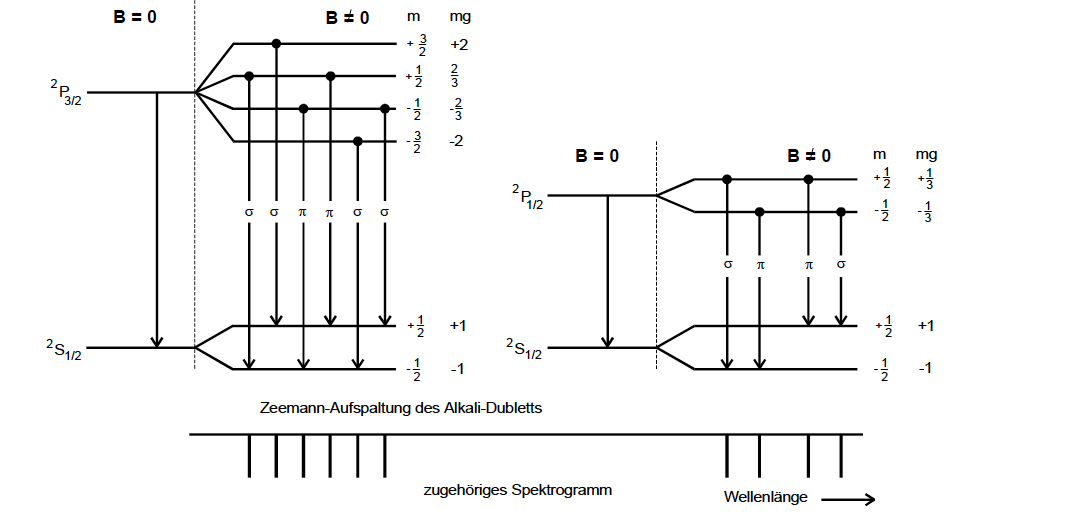
\includegraphics[scale=0.5]{anomal.PNG}
  \caption{Aufspaltung der Spektrallinien beim anomalen Zeeman- Effekt. \cite{Q1}}
  \label{abb3}
\end{figure}
\FloatBarrier

\subsection{Übergänge der Cadmiumlampe}
Im Versuch werden Übergänge in der Cadmium Lampe untersucht. Zum Einen die Aufspaltung der roten
und zum Anderen die Aufspaltung der blauen Spektrallinie.
Die rote Linie besitzt eine Wellenlänge von $\SI{643,8}{\nano\meter}$ und wird durch einen
Übergang von ${}^1P_1\leftrightarrow{}^1D_2$ hervorgerufen. Die blaue Linie besitzt
hingegen eine Wellenlänge von $\SI{480}{\nano \meter}$ und wird durch den Übergang von
${}^1S_1\leftrightarrow{}^3P_1$ hervorgerufen.
Der Übergang in der roten Spektrallinie entspricht dem normalen Zeeman- Effekt und die
blaue dem anomalen Zeeman- Effekt.
Die zu den jeweilogen Übergängen gehörenden Landé- Faktoren sind in Tabelle \ref{tab1} dargestellt.
\FloatBarrier

\begin{table}
    \centering
    \begin{tabular}{c c c c c c}
        \toprule
         &  $\multicolumn{2}{c}{${}1D_2$}$  &  $\multicolumn{2}{c}{${}^1P_1$} $  &  ${}^1P_1\leftrightarrow{}^1D_2$ \\
        %irgendwo schmeißt der hier noch einen Fehler, aber da blicke ich leider nicht so ganz drüber, da musst du nochmal gucken
        &  $ \multicolumn{2}{c}{${}1D_2$} $  &  $\multicolumn{2}{c}{${}^1P_1$} $ &  ${}^1P_1\leftrightarrow{}^1D_2$ \\
        &  $\multicolumn{2}{c}{${}1D_2$}$  &  $\multicolumn{2}{c}{${}^1P_1$}$  &  ${}^1P_1\leftrightarrow{}^1D_2$ \\

        \midrule
        Übergang & $m_{\alpha}$ & $g_{\alpha}$ & $m_{\beta}$ & $g_{\beta}$ & $g_{\alpha \beta}$ \\
        \midrule
        &   2   &   1   &   1   &   1   &   -1   \\
        $\sigma$  &  1  &   1   &   0   &   1   &   -1   \\
        &   0   &   1   &   -1  &   1   &   -1   \\
        \midrule
        &   1   &   1   &   1   &   1   &   0   \\
        $\pi$   &   0   &   1   &   0   &   1   &   0   \\
        &   -1   &   1   &  -1  &   1   &   0   \\
        \midrule
        &   0   &   1   &   1   &   1   &   1  \\
        $\sigma$    &   -1  &   1   &   0   &   1   &   1   \\
        &   -2  &   1   &   -1  &   1   &   1   \\
        \bottomrule
    \end{tabular}
    \caption{Orientierungsquantenzahlen und Landé- Faktoren für die rote Spektrallinie.}
    \label{tab1}
\end{table}
\FloatBarrier
\begin{table}
    \centering
    \begin{tabular}{c c c c c c}
        \toprule
%<<<<<<< HEAD:V27/V27.tex
        %&\multicolumn{2}{c}{${}^3S_1$} & \multicolumn{2}{c}{${}3P_1$}
        %auch hier stimmt irgendwas nicht
        &$ \multicolumn{2}{c}{${}^3S_1$} $ & $ \multicolumn{2}{c}{${}3P_1$}$

        & $\multicolumn{2}{c}{${}^3S_1$} $ & $\multicolumn{2}{c}{${}3P_1$}$
        \midrule
        Übergang    &   $m_{\alpha}$ & $g_{\alpha}$ & $m_{\beta}$ & $g_{\beta}$ & $g_{\alpha \beta}$ \\
        \midrule
        &   1   &   2   &   0   &   $\frac{3}{2}$   &   2   \\
        $\sigma$    &   0   &   2   &   -1  &   $\frac{3}{2}$   &   $\frac{3}{2}$   \\
        \midrule
        &   1   &   2   &   1   &   $\frac{3}{2}$   &   $\frac{1}{2}$   \\
        $\pi$   &   0   &   2   &   0   &   $\frac{3}{2}$   &   0   \\
        &   -1   &   2   &   -1   &   $\frac{3}{2}$   &   -$\frac{1}{2}$   \\
        \bottomrule
    \end{tabular}
    \caption{Orientierungsquantenzahlen und Landé-Faktoren für die blaue Spektrallinie.}
    \label{tab2}
\end{table}

\section{Aufbau und Durchführung}
\FloatBarrier
\begin{figure}
  \centering
  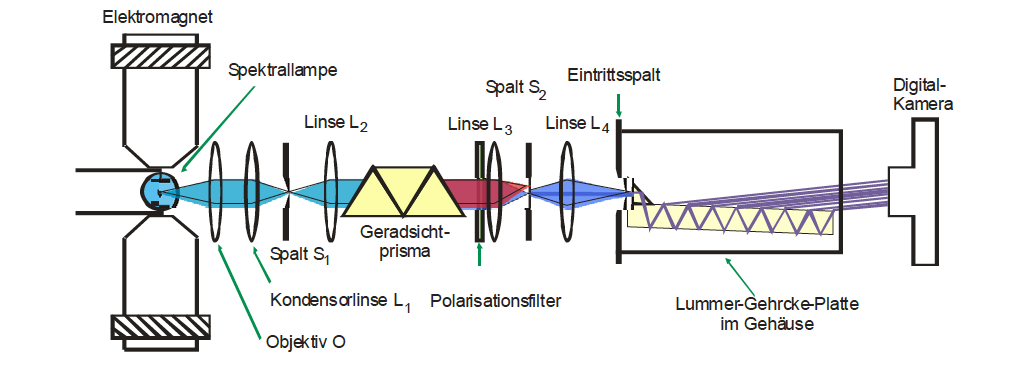
\includegraphics[scale=0.5]{aufbau.PNG}
  \caption{Schematischer Versuchsaufbau. \cite{Q1}}
  \label{abb4}
\end{figure}
\FloatBarrier

In Abbildung \ref{abb4} ist der schematische Versuchsaufbau zu sehen. Die Cadmiumlampe
wird im Versuch zwischen die Polschuhe eines Elektromagneten gestellt und gleich zu
Beginn des Versuchs eingeschaltet, damit sie ausreichend aufgewärmt ist.
Der Lichtstrahl der Cd-Lampe wird dann zunächst durch ein Objektiv und eine Sammellinse (L1)
geschickt. Hierbei ist darauf zu achten, dass durch diese Linse ein möglichst scharfes
Bild der Cd-Lampe auf dem Spalt (S1) abgebildet wird. Die Linse L2 dient dazu das Lichtbündel
auf das Geradsichtprisma abzubilden, sodass der Strahl das Prisma best möglich bedeckt.
Mit Hilfe der Linse L3 werden die aufgespalteten Spektrallinien möglichst scharf auf den
Spalt S3 abgebildet, mit dem im ersten Versuchsteil die rote Spektrallinie und im zweiten
Versuchsteil die blaue Spektrallinie ausgewählt wird. Dies geschieht, indem man die jeweilige
Linie exakt durch den Spalt durchlässt. Hier ist zu erwähnen, dass es hilfreich sein kann, die
Breite des Spaltes beim untersuchen der blauen Linie etwas zu verkleinern, um die, sehr nah neben
der blauen Linie liegende, Violette Linie auszublenden.
Mit Hilfe des Polarisationsfilters kann zwischen horizontaler und longitudinaler Betrachtung durch
Verschiebung um $\frac{\pi}{2}$ gewechselt werden. Die Position des Filters spielt für die Durchführung
keine Rolle. Um den Strahlengang nicht zu sehr zu beeinflussen, ist es jedoch von Vorteil, den Filter
kurz vor der Lummer-Gehrcke-Platte zu platzieren.
Das Lichtbündel wird anschließend durch eine Lummer-Gehrcke-Platte geschickt, welche durch
Totalreflexion an ihren Kanten und Intereferenz der Lichtstrahlen das Auflösungsvermögen erhöht.
Hierbei ist zu beachten, dass sich zwei Wellenlängen nicht überlagern sollen. Deshalb deren
Wellenlängendifferenz nicht größer als das Dispersionsgebiet der Lummer-Gehrcke-Platte sein:
\begin{align*}
    \Delta \lambda_D =\frac{\lambda^2}{2d}\sqrt{\frac{1}{n^2-1}}
    \label{eq:dis}
\end{align*}
In dieser Formel beschreibt $n$ den Brechungsindex und $d$ die Dicke der Platte.
Mit den gegebenen Daten für $n$ und $d$ für die Platte lässt sich nach der Berechnung von
$\Delta \lambda$ dann auch das Auflösungsvermögen $A$ der Lummer-Gehrcke-Platte berechnen:
\begin{align*}
    A = \frac{\lambda}{\Delta\lambda}=\frac{L}{\Lambda}(n^2-1)
\end{align*}
Vor Beginn des Versuchs werden zunächst alle Eigenschaften der Lummer-Gehrcke Platte berechnet.
Die Ergebnisse hierzu befinden sich in Tabelle \ref{tab3}.

\begin{table}
    \centering
    \begin{tabular}{ccccc}
		\toprule
		Farbe & $\lambda/\si{\nano\meter}$& $n$ & $\Delta\lambda_D/\si{\nano\meter}$& $A$\\\midrule
		rot & $\num{643,8}$ & $\num{1,4567}$ & $\num{489,1}$ & $\num{209e3}$\\
		blau & $\num{480,0}$& $\num{1,4635}$ & $\num{269,5}$ & $\num{285e3}$\\\bottomrule
\end{tabular}
    \caption{Eigenschaften der Lummer-Gehrcke-Platte.}
    \label{tab3}
\end{table}

\noindent Nachdem die Linsen justiert und ein Strahl ausgewhählt wurde(erst die rote,
dann die blaue Linie), wird zunächst
mit der vorhandenen Digitalkamera ein Bild der Spektrallinie ohne Magnetfeld aufgenommen.
Hierbei ist darauf zu achten, dass auf Grund des parallelen Strahlengang des Lichtes der
Fokus der Kamera auf $\infty$ gestellt ist und eine Belichtungszeit zwischen $5$ und
$\SI{10}{\second}$ gewählt wird.
Sodann wird das Magnetfeld aufgedreht, bis eine deutliche Aufspaltung der Spektrallinien
zu sehen ist. Nun wird ein Foto der aufegspaltenen Spektrallinie aufgenommen und die Magnetfeldstärke
notiert. Das Vorgehen ist bei roter, wie blauer Linie gleich, wobei zu erwähnen bleibt, dass die
Aufspaltung der blauen Linie etwas verwaschener im Bild erscheinen wird, was durch den Dopplereffekt
zu erklären ist.
Durch die verwendung der Lummer-Gehrcke-Platte sind im Fokus der Kamera sehr viele Spektrallinien zu sehen,
da hier ein Interferenzmuster entsteht. Es ist essentiell für die anschließende Auswertung, dass Messungen
der Wellenlängenänderung immer an derselben Linie durchgeführt werden, beziehungsweise dass bei der
Aufspaltung einer Linie in mehrere über deren Wellenlängenänderung gemittelt wird.
Nach Durchführung des Versuchs wird das Magnetfeld vermessen. Hierzu wird der Gleichstrom,
der den Permanentmagneten versorgt in $\SI{1}{\ampere}$-Schritten bis zu $\SI{1}{\ampere}$ hochgeregelt und zu
jeder Stromstärke das Magnetfeld mittels Hall-Sonde vermessen.



\section{Auswertung}
%gucken Punkte Komma
\subsection{Eichung des Elektromagneten}
Um die Magentfeldstärke im Inneren des Elektromagneten zu bestimmen, wird eine nichtlineare Regression der Form

\begin{equation}
  B(I) = a_0 + a_1 \cdot I + a_2 \cdot I² + a_3 \cdot I³
  \label{eq:B}
\end{equation}
durchgeführt. Diese liefert die Werte der Koeffizienten:

\begin{align*}
  a_0 &= \SI{5(5)}{\milli\tesla} \\
  a_1 &= \SI{59.0(18)}{\milli\tesla\per\ampere} \\
  a_2 &= \SI{0.80(19)}{\milli\tesla\per\ampere²} \\
  a_3 &= \SI{-0,053(6)}{\milli\tesla\per\ampere³}
\end{align*}
Die Messwerte und der Fit sind in Abbildung \ref{abb:1} und Tabelle \ref{tab:1} zu sehen.

\begin{table}
  \centering
  \caption{Messwerte zur Eichung des Elektromagneten.}
  \label{tab:1}
  \begin{tabular}{c c | c c}
    \toprule
    $I$ / \si{\ampere} & $B$ / \si{\milli\tesla} & $I$ / \si{\ampere} & $B$ / \si{\milli\tesla} \\
    \midrule
    0 & 4  & 12 & 742 \\
    1 & 62 & 13 & 806 \\
    2 & 124 & 14 & 839 \\
    3 & 197 & 15 & 891 \\
    4 & 250 & 16 & 935 \\
    5 & 307 & 17 & 980 \\
    6 & 379 & 18 & 1018 \\
    7 & 434 & 19 & 1050 \\
    8 & 509 & 20 & 1079 \\
    9 & 552 & 21 & 1108 \\
    10 & 611& 22 & 1132 \\
    11 & 680 \\
    \bottomrule
  \end{tabular}
\end{table}

\begin{figure}
  \centering
  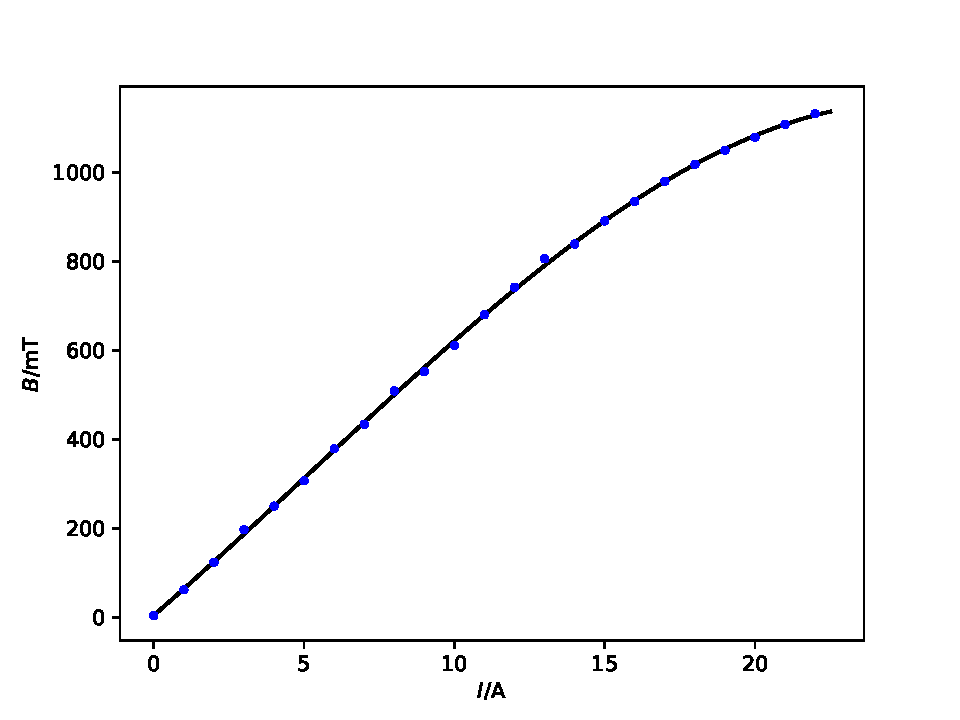
\includegraphics[scale=0.7]{Magnetfeld.pdf}
  \caption{Fit und Messwerte zur Eichung des Elektromagneten.}
  \label{abb:1}
\end{figure}


\subsection{\texorpdfstring{Zur Berechnung der $\symup{\Delta}(m \cdot g)$}{}-Werte}
Die bekannte Formel
\begin{equation*}
  E(\lambda) = \frac{hc}{\lambda}
\end{equation*}
zur Berechnung der Energie einer elektromagnetischen Welle aus deren Wellenlänge $\lambda$
sowie dem $\textsc{Planck}$schen Wirkungsquantum $h$ und der Vakuumlichtgeschwindigkeit $c$
ist offensichtlich nicht linear in $\lambda$. Da für diese Auswertung jedoch ein Wert
$\symup{\Delta} E(\symup{\Delta} \lambda)$ notwendig ist um nach:
\begin{equation}
  \symup{\Delta} E = \underbrace{ \{m_1 g_1 - m_2 g_2 \} }_{\substack{\symup{\Delta}(m \cdot g)}}
  \mu_B B
  \label{eq:2}
\end{equation}
aus einer Magnetfeldstärke $B$ und dem $\textsc{Bohr}$schen Magenton einen Wert $\symup{\Delta}(m \cdot g)$
zu berechnen, muss die Ableitung $\frac{\partial}{\partial \lambda} E$ bestimmt werden da
ein Gleichsetzen der beiden Ausdrücke für $E$ aufgrund der erwähnten nicht-Linearität verboten ist.
Aus der Ableitung folgt:
\begin{equation}
  \frac{\partial}{\partial \lambda} E = -\frac{h c}{\lambda^2} \Leftrightarrow
  \symup{\Delta} E = -\frac{h c}{\lambda^2} \symup{\Delta} \lambda.
  \label{eq:3}
\end{equation}
Dieser Ausdruck ist nun abhängig von der konstanten unverschobenen Wellenlänge
$\lambda$ und linear in der Wellenlängenverschiebung $\symup{\Delta} \lambda$. Ein Gleichsetzen der
Ausdrücke \eqref{eq:2} und \eqref{eq:3} ist daher erlaubt und liefert:
\begin{equation}
  |\symup{\Delta}(m \cdot g)| = \frac{h c}{\lambda^2 \mu_B B} \symup{\Delta} \lambda.
  \label{eq:4}
\end{equation}


\subsection{Auswertung der roten Linie}

Zur Auswertung werden die Abstände $\symup{\Delta} s$ der Linien ohne Magnetfeld und die Abstände $\symup{\delta} s$ der aufgespaltenen Linien mit Magnetfeld ausgemessen.
Da der Abstand zwischen zwei Linien vermessen wird, aber sich je eine Linie durch das Magnetfeld in zwei aufspaltet, muss der Mittelwert der jeweils
angrenzenden $\symup{\delta} s$ genommen werden. Die Abstände sind in Tabelle \ref{tab:2} aufgelistet, wobei die Einheit der Abstände Pixel beschreibt.
Das Dispersionsgebiet wird mit der Formel \eqref{eq:dis} berechnet, wobei hier die Wellenlänge $\lambda= \SI{643,8}{\nano\meter}$, die Dicke der
Lummer-Gehrcke-Platte $L=\SI{4}{\milli\meter}$ und der dazugehörige Brechungsindex $n(\SI{643,8}{\nano\meter})= 1,4567$ eingesetzt wird:

\begin{equation*}
  \symup{\Delta}\lambda_{\symup{D, rot}} = \SI{48,91}{\pico\meter}
\end{equation*}

Die Wellenlängenänderung $\symup{\delta}\lambda$ kann somit durch die Formel

\begin{equation}
\symup{\delta}\lambda = \frac{1}{2} \frac{\symup{\delta}s}{\symup{\Delta}s} \cdot \symup{\Delta}\lambda_{\symup{D}}
\label{eq:5}
\end{equation}

berechnet werden. Die berechneten Wellenlängenverschiebungen $\symup{\delta}\lambda$
sind ebenfalls in Tabelle \ref{tab:2} zu finden.
Der Mittelwert der Wellenlängenverschiebung beträgt
$\overline{\symup{\delta}\lambda_{·\symup{rot}}} = \SI{10.89(15)}{\pico\meter}$.

Zu Berechnung des dazugehörigen Landé-Faktors muss die Magnetische Feldstärke B
mit Hilfe der Ausgleichsrechnung zur Eichung des Magnetfeld berechnet
werden (siehe Gleichung \eqref{eq:B})
\begin{equation*}
  B(\SI{9}{\ampere})= \SI{561,64}{\milli\tesla}
\end{equation*}

Der Landé-Faktor kann nun mit Hilfe der Formel \eqref{eq:4} bestimmt werden:

\begin{equation}
  |\symup{\Delta}(m \cdot g)| = \frac{h c}{\lambda^2 \mu_B B} \symup{\Delta} \lambda.
  \label{eq:lande}
\end{equation}

Mit dem $\textsc{Planck}$schen Wirkungsquantum $h$, der Vakuumlichtgeschwindikeit
$c$, der Wellenlänge $ \lambda = \SI{643,8}{\nano\meter}$, dem Bohrschen
Magneton $\mu_B$ und der Wellenlängeverschiebung $\symup{\Delta}\lambda$ folgt

\begin{equation*}
  |\symup{\Delta}(m \cdot g)_{\symup{rot, \sigma}}| = \SI{1,002(5)}{}.
\end{equation*}

Da es bei dem normales Zeeman-Effekt keine Verschiebung der Linie bei dem
$\pi$-Übergang, wird hier $|\symup{\Delta}(m \cdot g)_{\symup{rot, \pi}}| = 0$
angenommen.

\begin{table}
  \centering
  \caption{Messwerte: Abstände der roten Linie.}
  \label{tab:2}
  \begin{tabular}{c c c}
    \toprule
    $\symup{\Delta}s$ / pix & $\symup{\delta}s$ / pix & $\symup{\delta}\lambda$ / \si{\pico\meter} \\
    \midrule
    392.00 & 170.50 & 10.64 \\
    333.00 & 148.50 & 10.91 \\
    301.00 & 132.50 & 10.77 \\
    267.00 & 118.50 & 10.85 \\
    247.00 & 112.00 & 11.09 \\
    230.00 & 104.00 & 11.06 \\
    220.00 & 97.00 & 10.78 \\
    209.00 & 94.50 & 11.06 \\
    196.00 & 88.50 & 11.04 \\
    193.00 & 83.50 & 10.58 \\
    177.00 & 78.00 & 10.78 \\
    158.00 & 72.00 & 11.14 \\
    \bottomrule
  \end{tabular}
\end{table}

\begin{figure}
\begin{subfigure}[c]{0.5\textwidth}
  
\includegraphics[width=\textwidth]{Bild1.JPG}
  \subcaption{B=0}
\end{subfigure}
\begin{subfigure}[c]{0.5\textwidth}
  
\includegraphics[width=\textwidth]{Bild2.JPG}
  \subcaption{B$\neq$0}
\end{subfigure}
\caption{Aufspaltung der roten Linie.}
\end{figure}


\subsection{Auswertung der blauen Linie}

Zur Auswertung des anormalen Zeeman-Effekts bei der blauen Linie, werden erneut
die Abstände $\symup{\Delta}s$ der Linien ohne Magnetfeld gemessen und
anschließend die Abstände $\symup{\delta}s$ zwischen den durch das Magnetfeld
aufgespalteten Linien. Auch hier muss der Mittelwert der angrenzenden
$\symup{\delta}s$ genommen werden.
Zur Berechnung der Wellenlängenverschiebung muss zunächst das
Dispersiongebiet mit Hilfe der Gleichung \eqref{eq:dis} berechnet werden.
\begin{equation*}
  \symup{\Delta}\lambda_{\symup{D, blau}} = \SI{26.95}{\pico\meter}
\end{equation*}

Die Messwerte und die mit Gleichung \eqref{eq:5} berechneten
Wellenlängeverschiebungen sind in Tabelle \ref{tab:2} aufgelistet.
Der Mittelwert der Wellenlängenverschiebung beträgt

\begin{align*}
  \overline{\symup{\delta}\lambda_{\symup{blau, \pi}}} &= \SI{6.25(17)}{\pico\meter} \\
  \overline{\symup{\delta}\lambda_{\symup{blau, \sigma}}} &= \SI{6.31(19)}{\pico\meter}
\end{align*}

Mit Hilfe der zuvor berechneten Regression für das Magnetfeld im Inneren des
Elektromagneten (siehe Gleichung \eqref{eq:B}) wird die Magentfeldstärke bestimmt:
\begin{align*}
  B(I_{\symup{blau, \pi}}=\SI{21}{\ampere}) &= \SI{1108.15}{\milli\tesla} \\
  B(I_{\symup{blau, \sigma}}=\SI{5.5}{\ampere}) &= \SI{344.31}{\milli\tesla} \\
\end{align*}

Nun können durch die Gleichung \eqref{eq:lande} die Landé-Faktoren berechnet werden.

\begin{align*}
  |\symup{\Delta}(m \cdot g)_{\symup{blau, \pi}}| = \SI{1.69(5)}{} \\
  |\symup{\Delta}(m \cdot g)_{\symup{blau, \sigma}}| = \SI{0.530(16)}{}.
\end{align*}

\begin{table}
  \centering
  \caption{Messwerte zur blauen Linie.}
  \label{tab:3}
  \begin{tabular}{c c c|c c c}
    \toprule
    \multicolumn{3}{c}{$\pi$-Übergang} & \multicolumn{3}{c}{$\sigma$-Übergang} \\
    $\symup{\Delta}s_{\pi}$ / pix & $\symup{\delta}s_{\pi}$ / pix & $\symup{\delta}\lambda_{\pi}$ / \si{\pico\meter} &
    $\symup{\Delta}s_{\sigma}$ / pix & $\symup{\delta}s_{\sigma}$ / pix & $\symup{\delta}\lambda_{\sigma}$ / \si{\pico\meter} \\
    \midrule
    380 & 155 & 5.50 & 306 & 168 & 7.40 \\
    308 & 140 & 6.12 & 280 & 132 & 6.35 \\
    208 & 124 & 8.03 & 242 & 115 & 6.40 \\
    238 & 106 & 6.00 & 228 & 101 & 5.97 \\
    222 & 96 & 5.83 & 210 & 97 & 6.22 \\
    216 & 94 & 5.86 & 204 & 96 & 6.34 \\
    188 & 92 & 6.59 & 246 & 89 & 4.88 \\
    184 & 91 & 6.66 & 184 & 80 & 5.86 \\
    178 & 86 & 6.51 & 162 & 76 & 6.32 \\
    168 & 80 & 6.42 & 166 & 74 & 6.01 \\
    158 & 73 & 6.23 & 144 & 70 & 6.55 \\
    148 & 66 & 6.01 & 135 & 67 & 6.69 \\
    \bottomrule
  \end{tabular}
\end{table}

\begin{figure}
 \begin{subfigure}[c]{0.5\textwidth}
   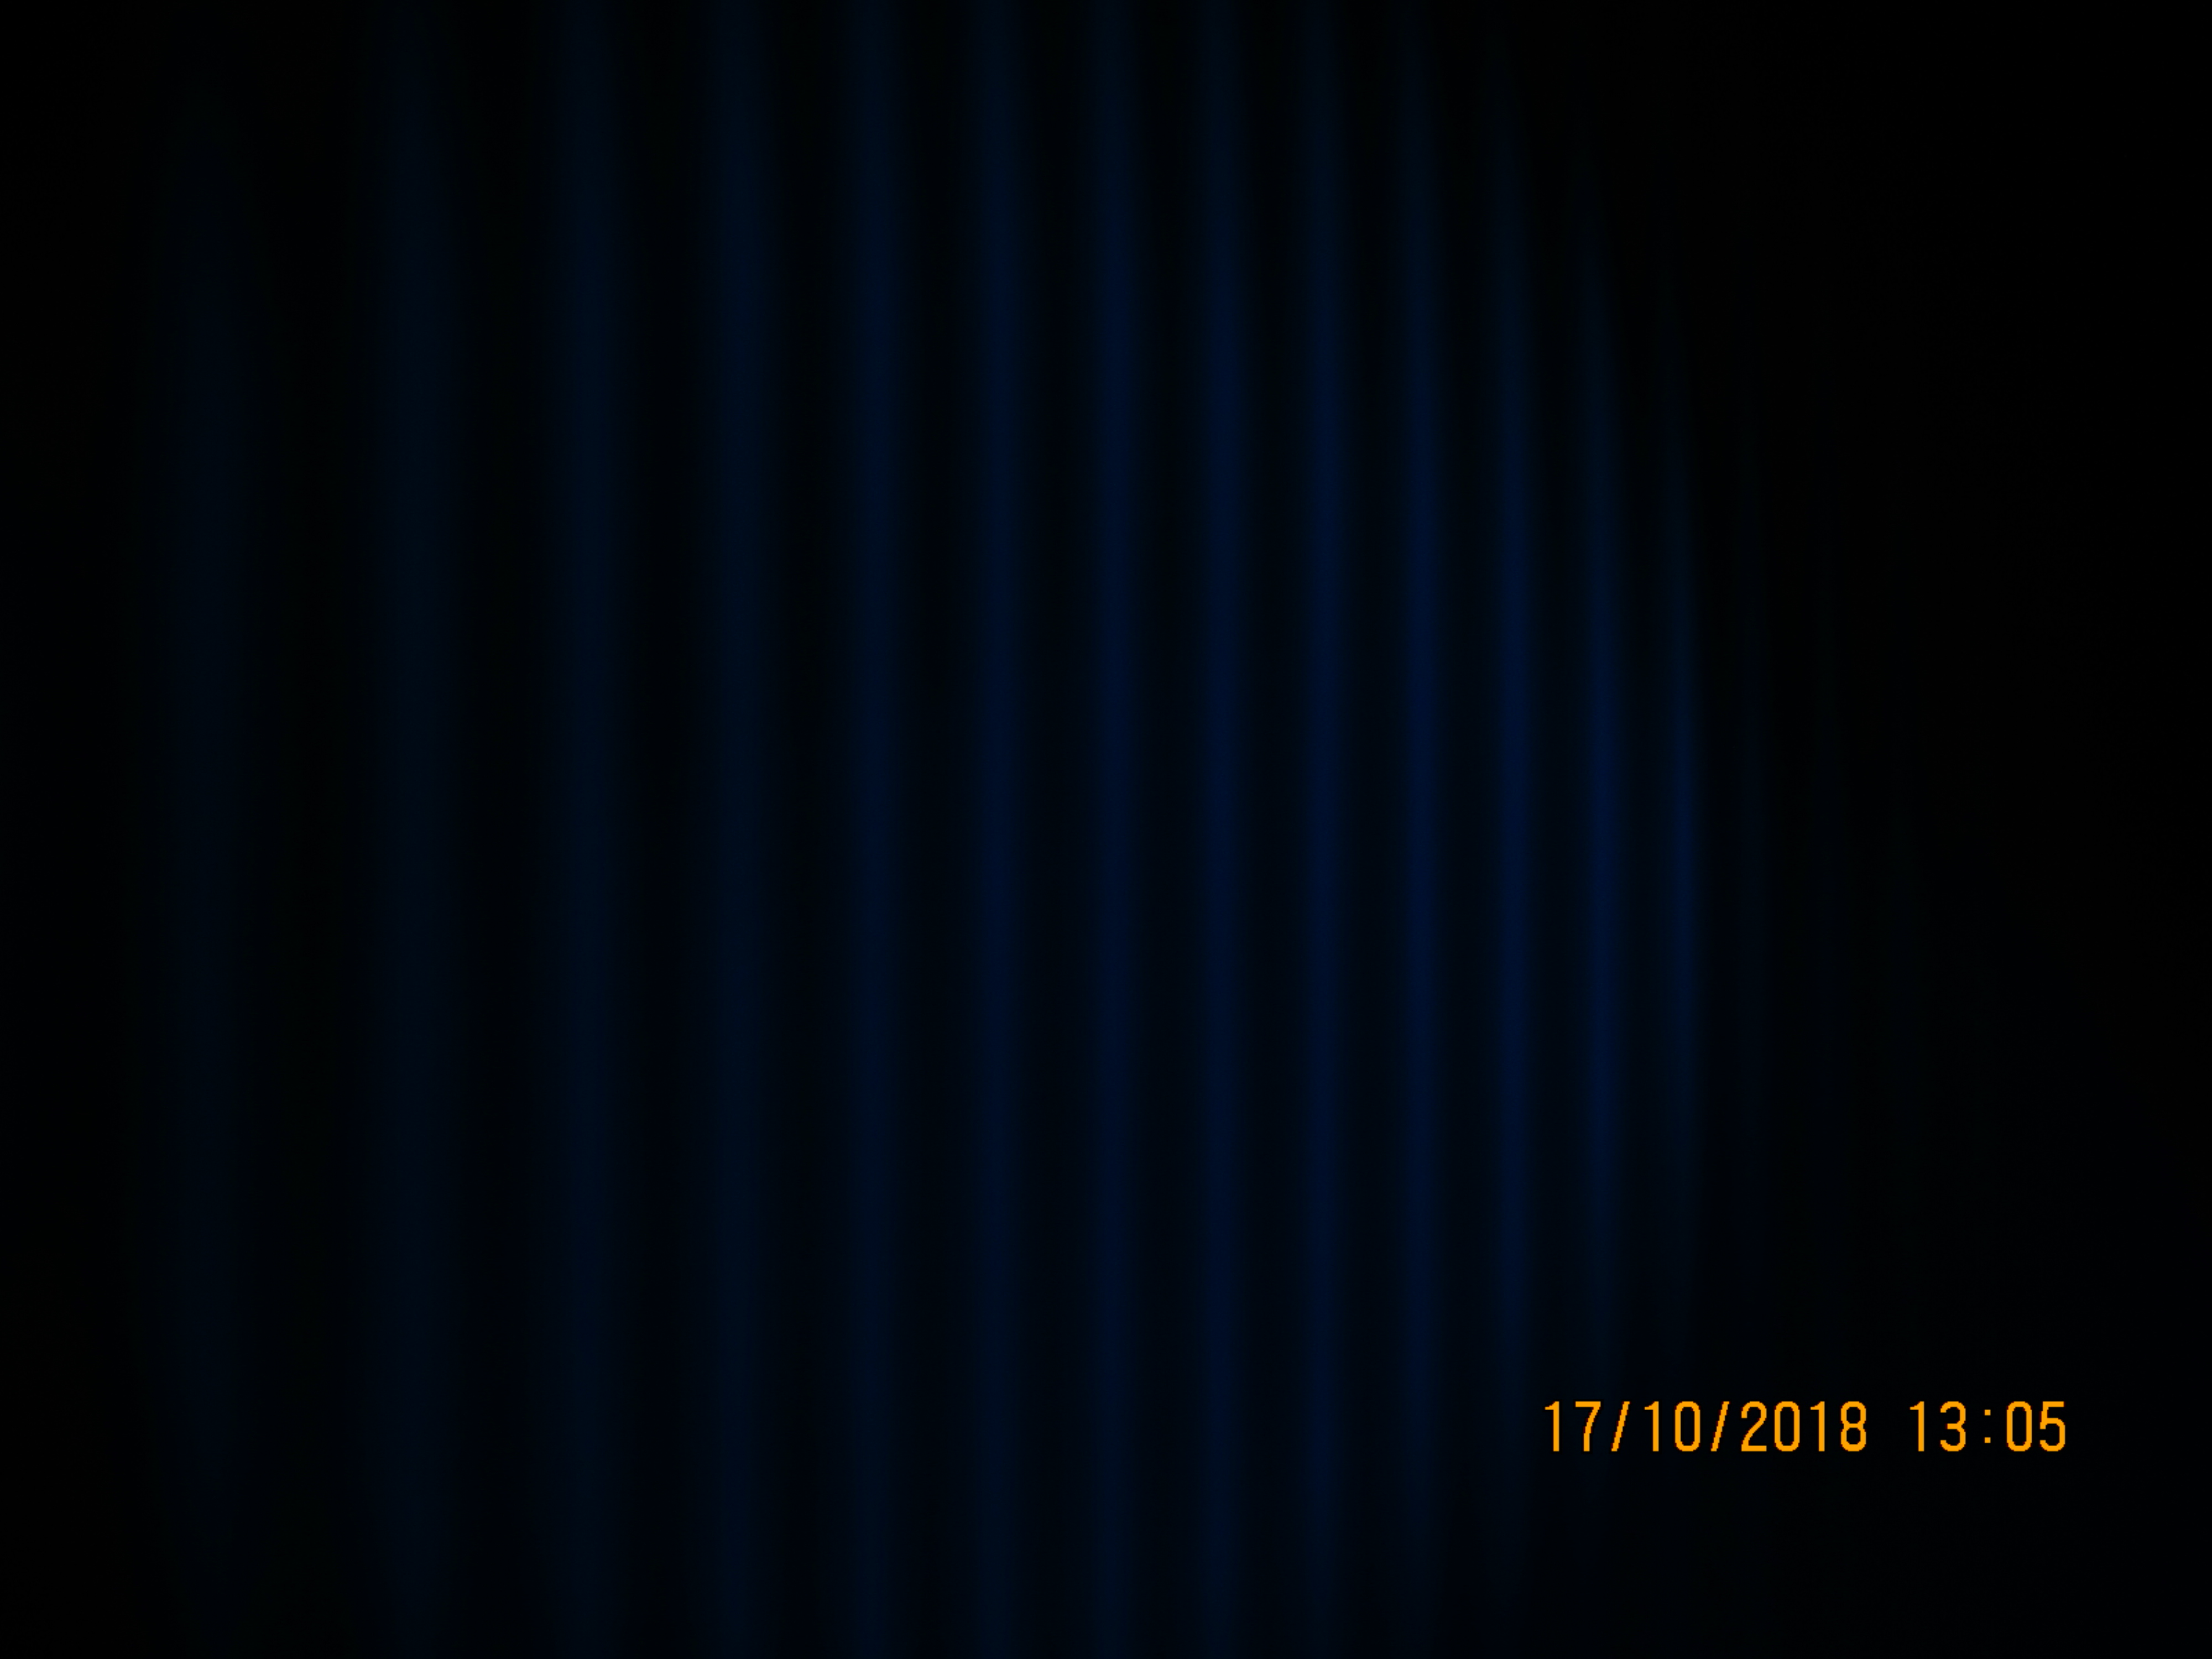
\includegraphics[width=\textwidth]{Bild8.JPG}
   \subcaption{B=0}
 \end{subfigure}
 \begin{subfigure}[c]{0.5\textwidth}
   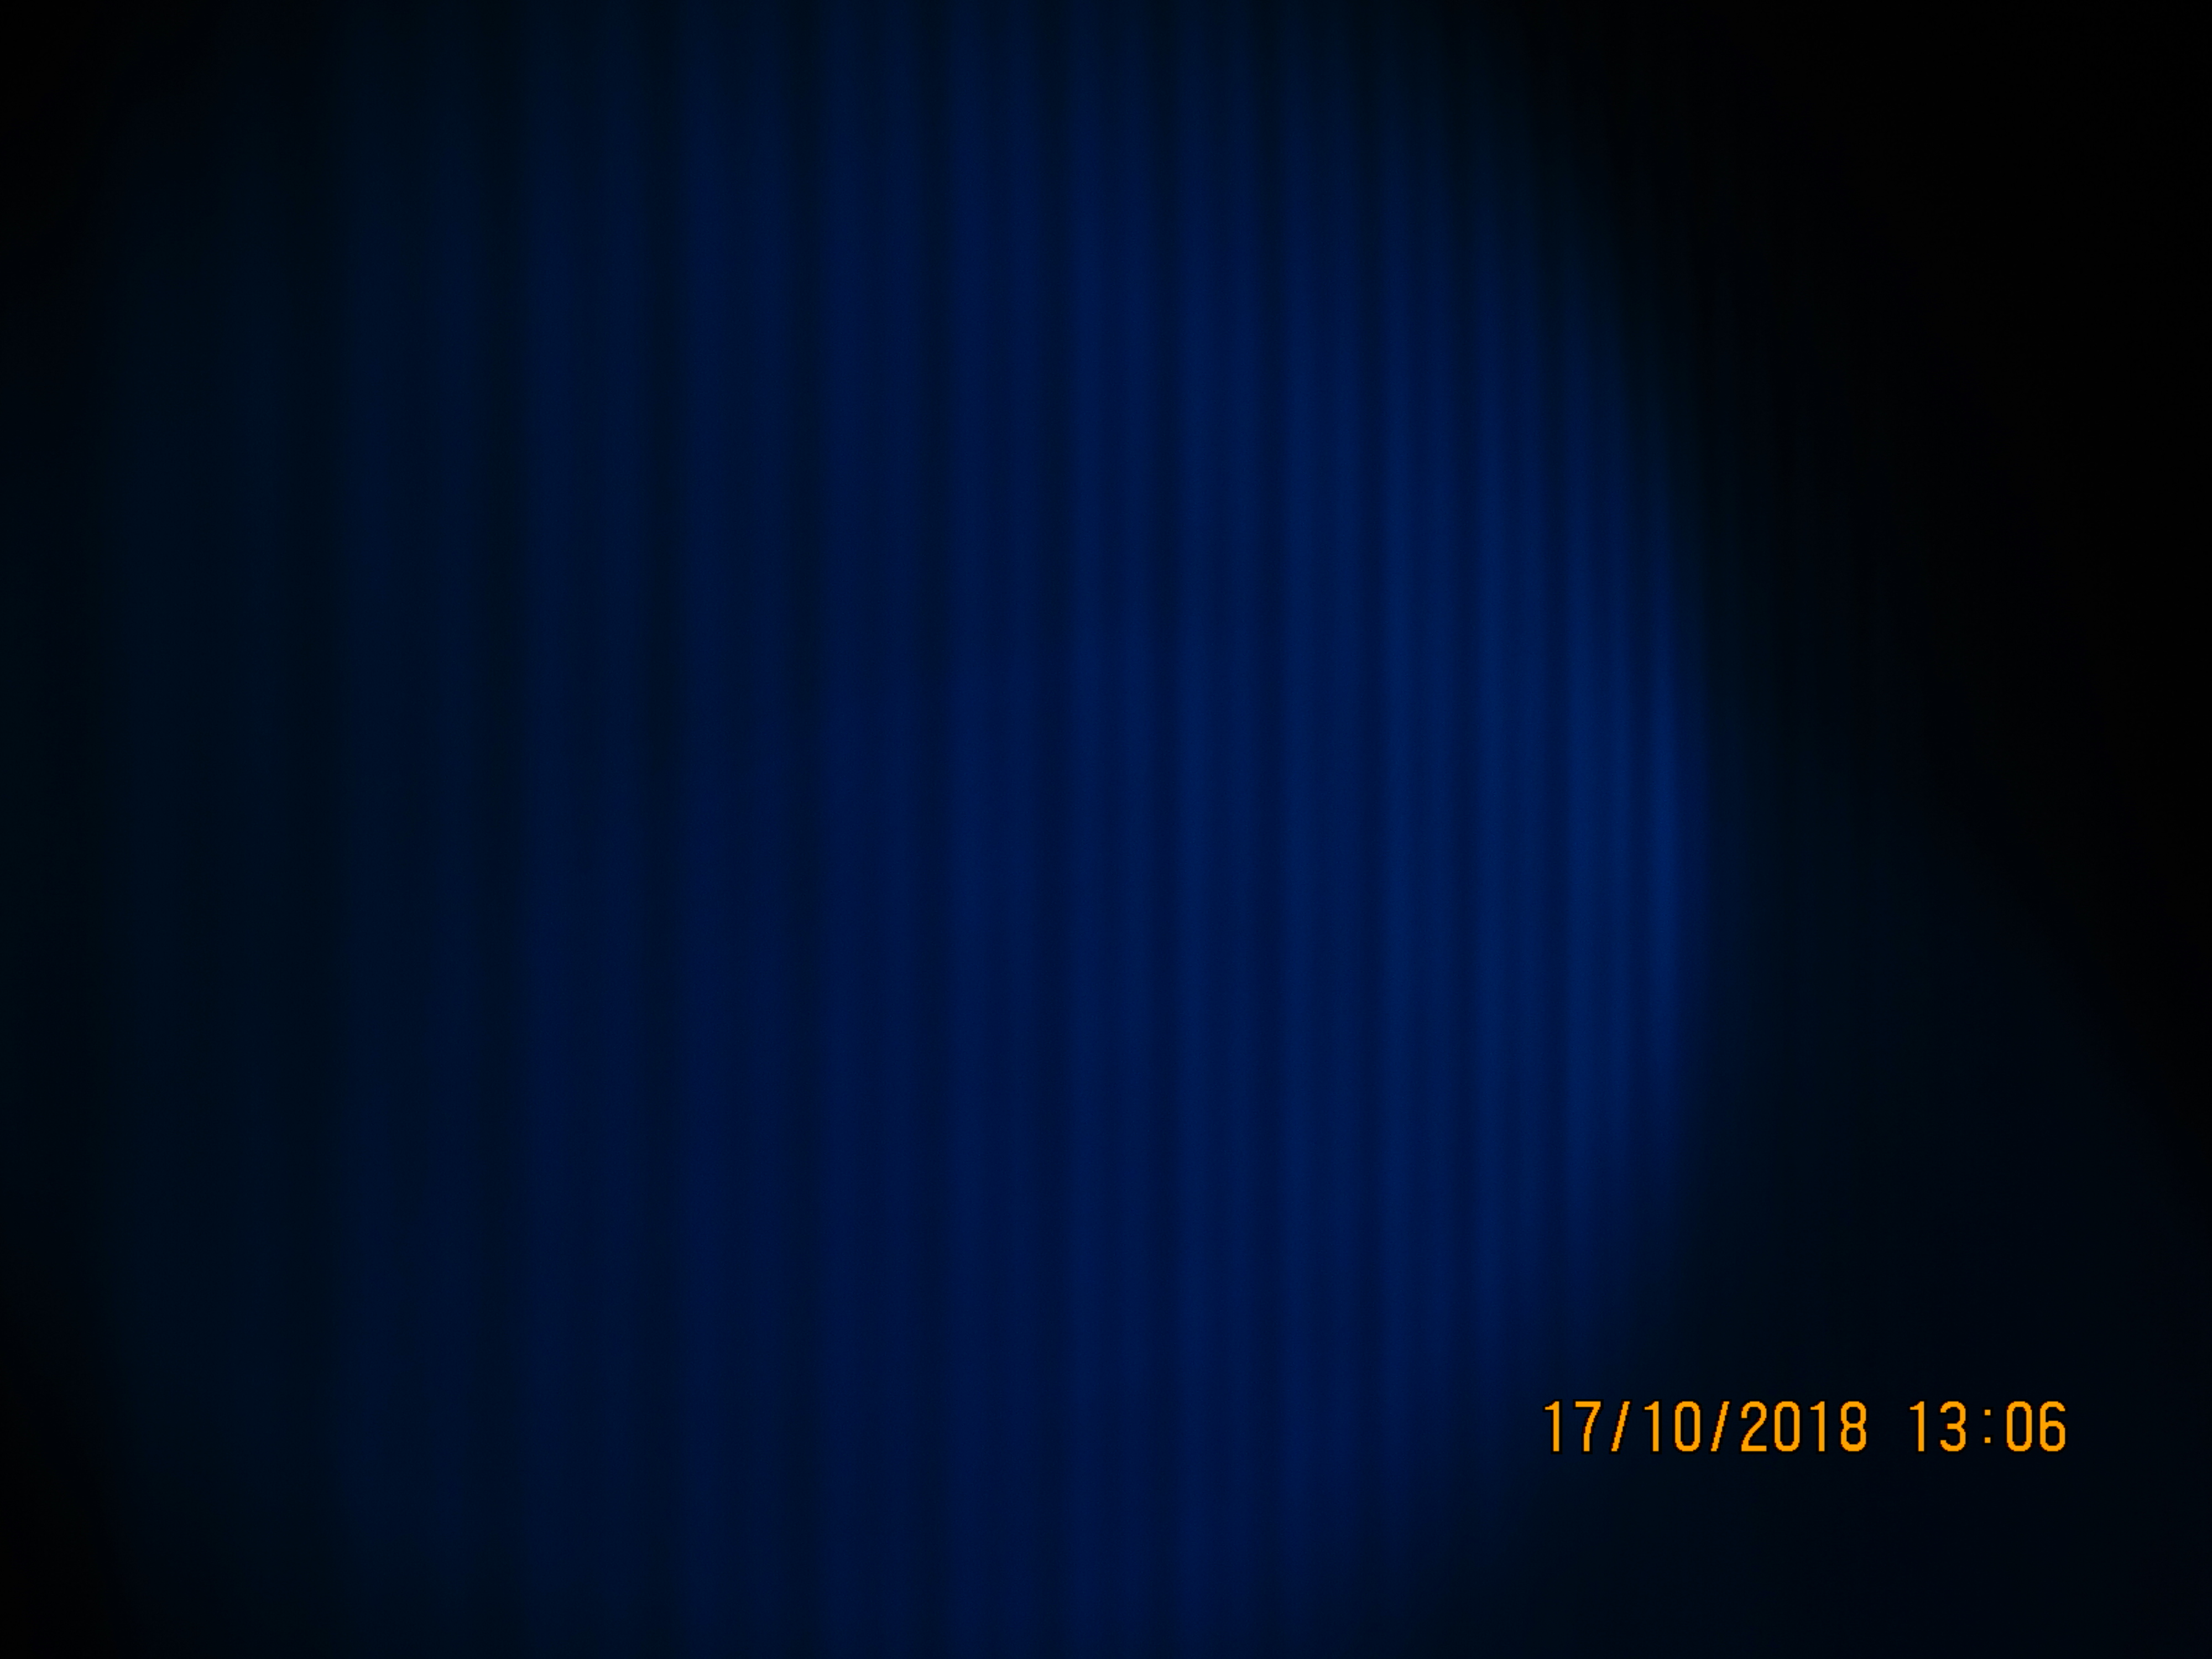
\includegraphics[width=\textwidth]{Bild9.JPG}
   \subcaption{B$\neq$0}
 \end{subfigure}
 \caption{Aufspaltung der blauen Linie für den $\pi$-Übergang.}
\end{figure}

\begin{figure}
 \begin{subfigure}[c]{0.5\textwidth}
   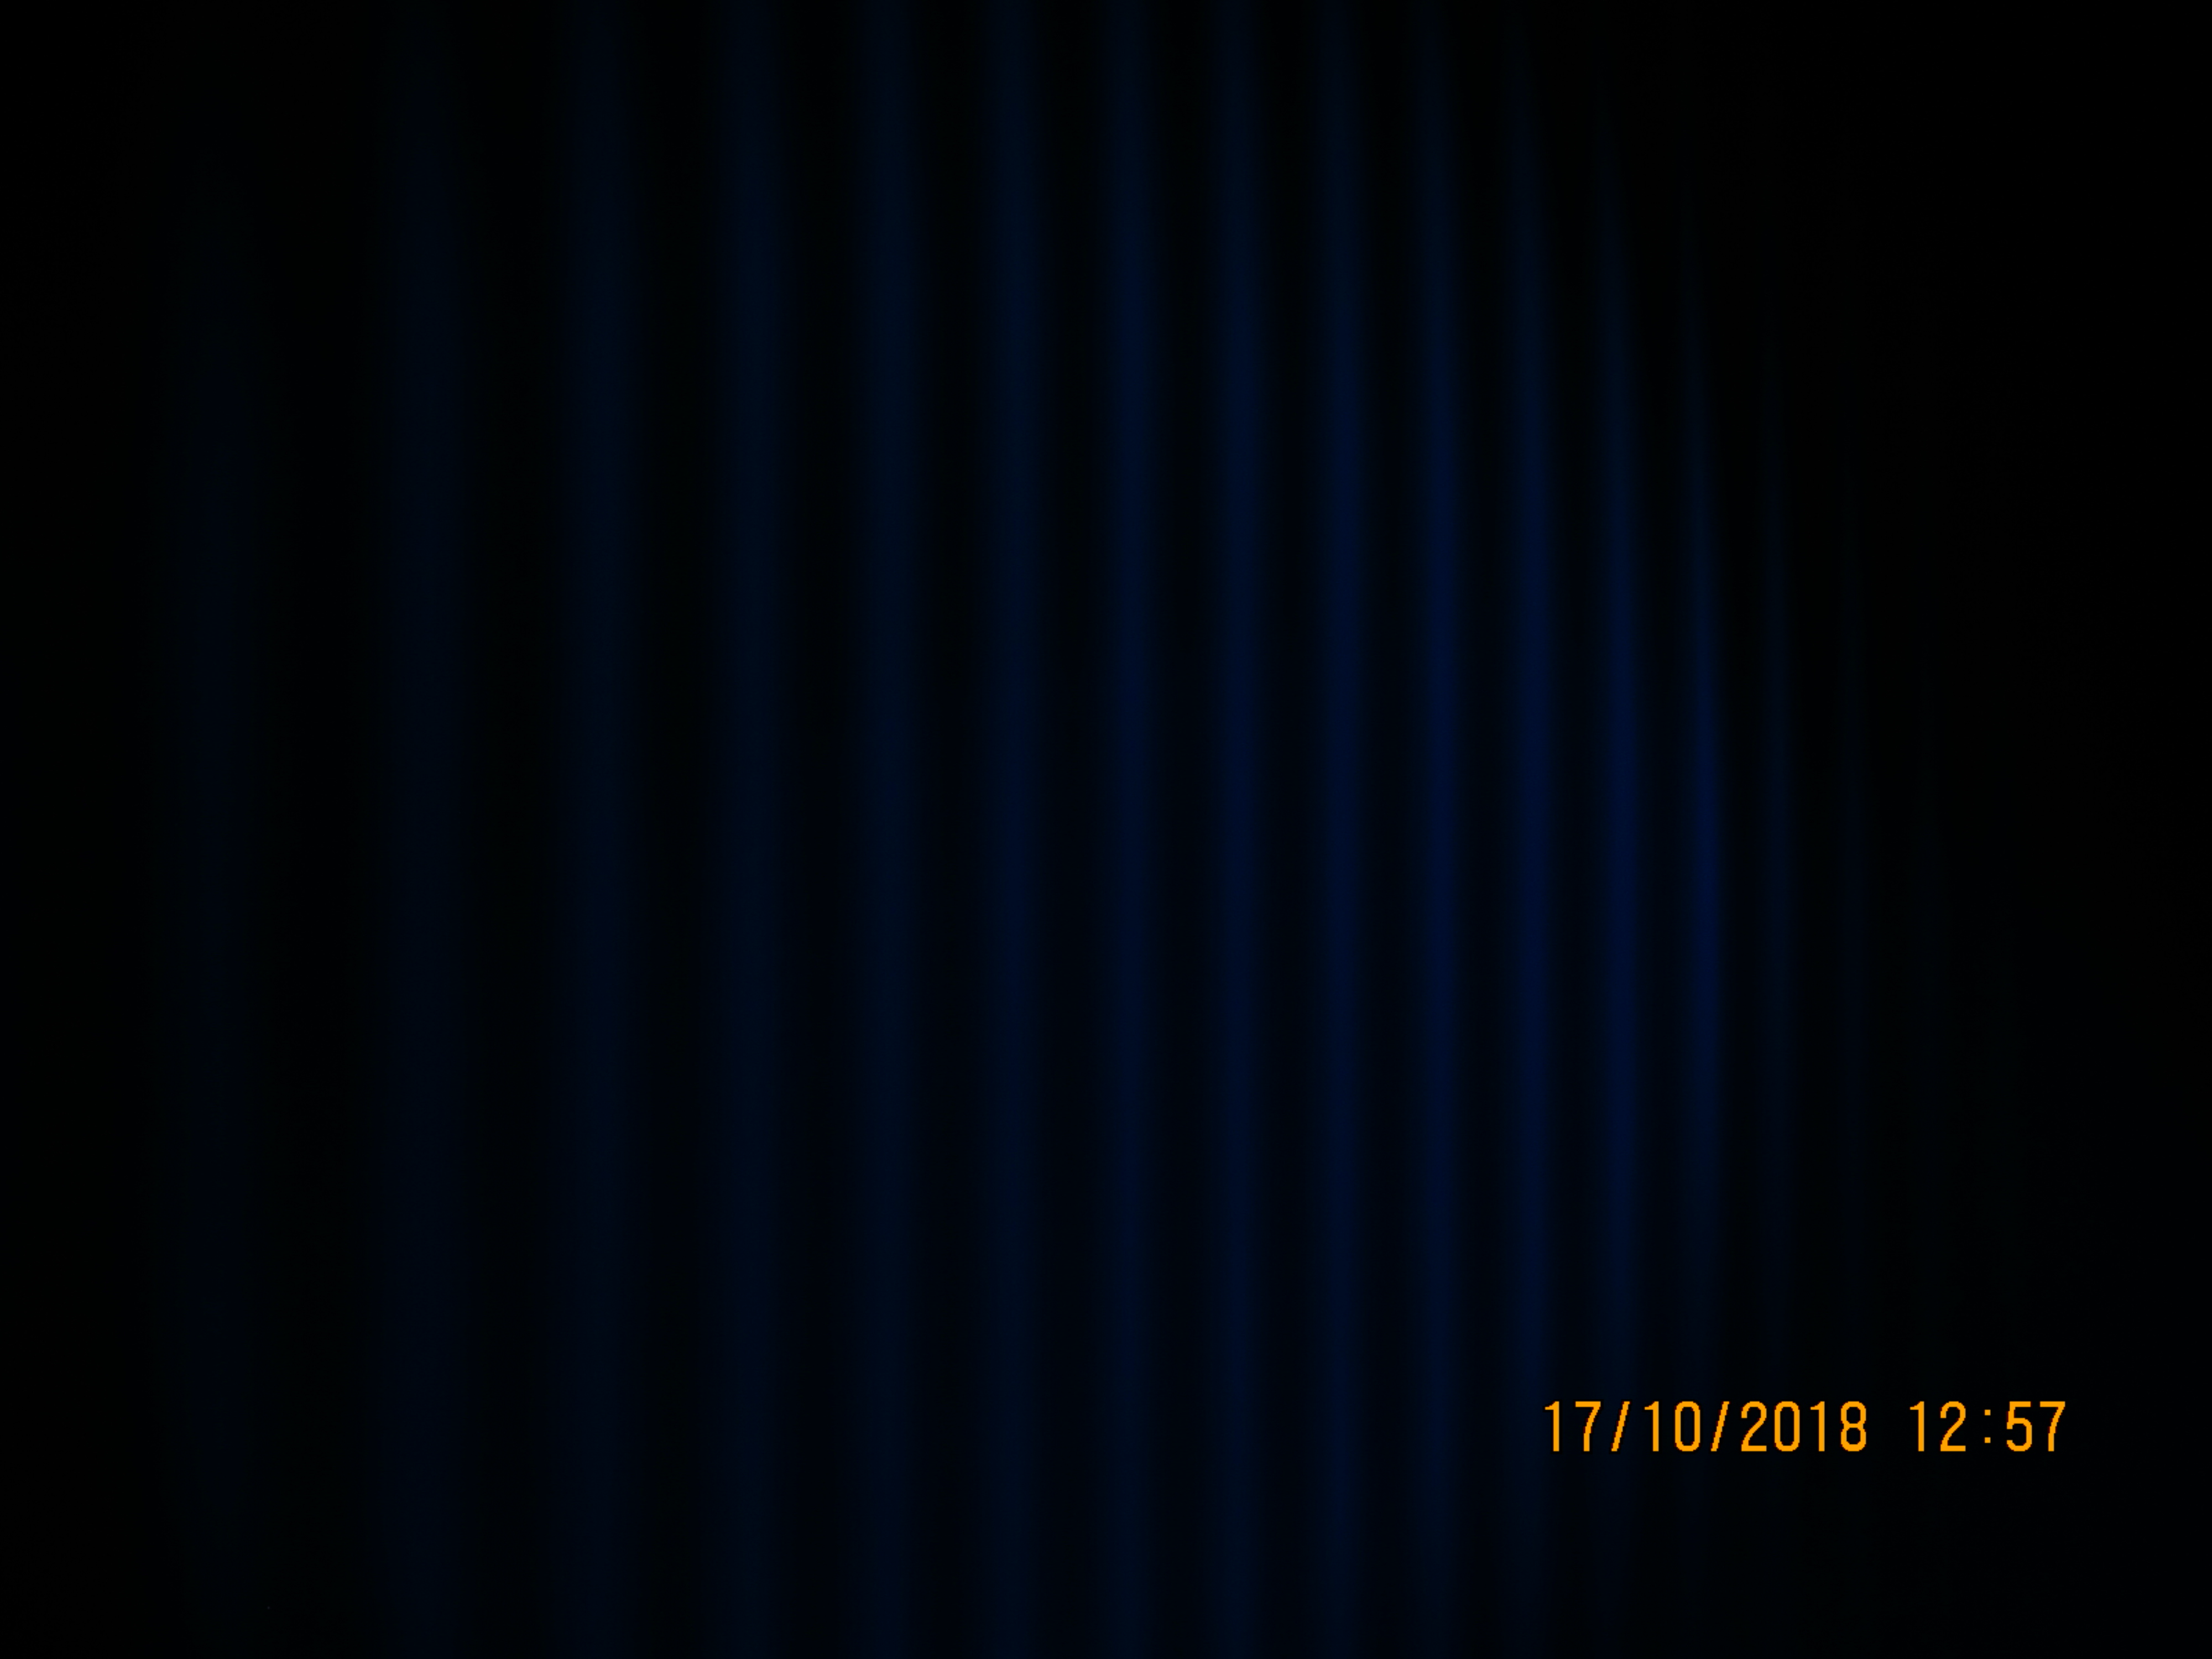
\includegraphics[width=\textwidth]{Bild4.JPG}
   \subcaption{B=0}
 \end{subfigure}
 \begin{subfigure}[c]{0.5\textwidth}
   
\includegraphics[width=\textwidth]{Bild6.JPG}
   \subcaption{B$\neq$0}
 \end{subfigure}
 \caption{Aufspaltung der blauen Linie für den $\sigma$-Übergang.}
\end{figure}

\section{Diskussion}

\begin{table}
  \centering
  \caption{Vergleich der Messwerte mit den Theoriewerten.}
  \label{tab:4}
  \begin{tabular}{c c c c}
    \toprule
    Übergäng & Theoriewert & Messwert & Abweichung \\
    \midrule
    rot, $\pi$ & 0 & 0 (nicht explizit berechnet) & - \\
    rot, $\sigma$ & 1 & 1.002\pm0.005 & \SI{0.2}{\percent}\\
    blau, $\pi$ & 1,75 & 1.69\pm0.05 & \SI{3.5}{\percent}\\
    blau, $\sigma$ & 0.5 & 0.530\pm0.016 & \SI{6}{\percent}\\
    \bottomrule
  \end{tabular}
\end{table}

Ein Vergleich der Theorie- und der Messwerte für den Landé-Faktor
$|\symup{\Delta}(m \cdot g)|$ findet sich in Tabelle \ref{tab:4}.
Für die rote Spektrallinie befindet sich der Theoriewert im Bereich der
Messungenauigkeit. Bei der blauen Spektrallinie befindet sich der
Theoriewert im zwar nicht in der Messungenauigkeit, aber in dem $2\sigma$-Intervall.
Da bei dem $\sigma$-Übergang eingentlich vier dünne Linien zu sehen sind mit Landé-Faktor
1,5 und 2, wird hier der Mittelwert als Theoriewert angenommen, da je zwei dieser
Linien so dicht beieinander liegen, dass diese mit dem Versuchsaufbau nicht zu
erkennen sind.
Als größte Fehlerquelle lässt sich das Ablesen der Abstände einordnen, denn die
Spektrallinien wurden nicht Scharf auf dem Foto abgebildet, sondern haben
ein Intensitätsmaximum, welches durch das bloße Auge abgemessen wurde, bzw.
durch setzen eines Markers am Computer. Dies lässt auf eine Ungenauigkeit
der Messwerte schließen.
Außerdem ist die Messung der Magnetfeldstärke mittels der Hallsonde auch
nicht vollkommen genau, da die Hallsonde nur das Magnetfeld misst, welches
senkrecht zu der Hallsonde verläuft, hierbei kann es also nur durch geringes
Drehen der Sonde zu Fehlern kommen.
Dennoch sind die Messwerte mit einer maximalen Abweichung von \SI{6}{\percent}
sehr genau bestimmt worden. Ein Grund hierfür ist die sehr hohe Auflösung
der Lummer-Gehrcke-Platte.
Generell entsprechen die Ergebnisse des Versuches der theoretischen Grundlage
des Zeeman-Effektes.
